\section{Introduction}

\begin{frame}
\huge{\centerline{Section 1: Introduction }}
\end{frame}
\begin{frame}
\frametitle{Binary Classification} % Table of contents slide, comment this block out to remove it
\begin{itemize}
\item Key problem in supervised machine learning.


%----------------------------------------------------------------------------------------
%	PRESENTATION SLIDES
%----------------------------------------------------------------------------------------

%------------------------------------------------
\item Predict binary output from input variables, e.g.
%Examples:
\begin{itemize}
\item[--] Spam or not spam
\item[--] Disease or no disease
\item[--] Rain or no rain
\item[--] Win or lose election etc.
\end{itemize}
%\section{Binary classification} % Sections can be created in order to organize your presentation into discrete blocks, all sections and subsections are automatically printed in the table of contents as an overview of the talk
%------------------------------------------------

%\subsection{Spam or not spam} % A subsection can be created just before a set of slides with a common theme to further break down your presentation into chunks
%\subsection{Disease or no disease etc.}
\item Simplest classifiers: linear classifiers, e.g. \textit{perceptron}.
\end{itemize}
\end{frame}
%------------------------------------------------
\begin{frame}
\frametitle{Linear classification}
\begin{figure}
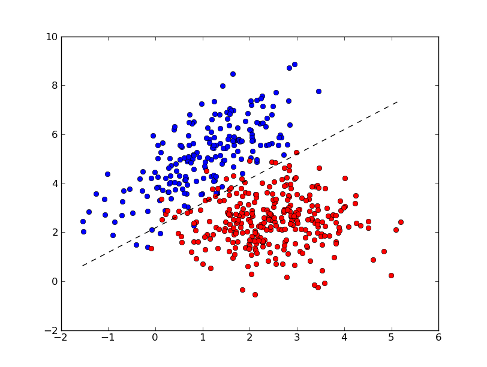
\includegraphics[width=0.6\linewidth]{lda_binary.png}
\caption{Example of linear classification}
\end{figure}
\end{frame}
%------------------------------------------------
\begin{frame}
\frametitle{Linear Classification}
\begin{itemize}
\item Output binary class (0 or 1) based on where a linear combination of the input feature vector lies with respect to the decision boundary:
\begin{equation}
y = \frac{1}{2}(1 + \text{sign} (\theta^T \mathbf{x}))
\end{equation}
$\mathbf{x} \in \mathds{R}^{d+1}, \theta \in \mathds{R}^{d+1}; y \in \{0,1\}.$\\

\begin{itemize}
\item[--] $ \theta^T \mathbf{x} = 0 \implies \text{decision boundary}$
\item[--] $ \theta^T \mathbf{x} > 0 \implies y = 1$
\item[--] $ \theta^T \mathbf{x}  < 0 \implies y = 0$
\end{itemize}

\item The decision boundary (i.e. $\theta$) is learned from the training data.
\end{itemize}
\end{frame}

\begin{frame}
\frametitle{Hard vs. Soft Threshold}
\begin{itemize}
\item Exact binary prediction (\textit{hard threshold}) may be impractical - does not reveal the confidence in the prediction.
% Talk about the non-linearity as well
\item Express as \textit{probability} of belonging to a class (\textit{soft threshold}), e.g. probability of raining, probability of a heart disease etc. \item Instead of a strict binary value, the classifier output is a real number between 0 and 1 - interpreted as class probability.
\item This leads to \textbf{logistic regression}.
\end{itemize}
\end{frame}

\begin{frame}
\frametitle{Modeling Conditional Probabilities}
\begin{itemize}
\item Determine a conditional probability distribution, or \textit{likelihood} $P(Y|X)$ that best describes the observed data.
\item Assuming $P(Y=1|X=\mathbf{x}) = p(\mathbf{x};\theta)$ for some function $p$ parameterized by $\theta$ and with $i.i.d.$ observation variables, the conditional likelihood function $P(Y|X)$ is,
\begin{equation}
\prod_{i=1}^n P(Y=y_i|X=\mathbf{x}_i) = \prod_{i=1}^n p(\mathbf{x}_i;\theta)^{y_i} (1-p(\mathbf{x}_i;\theta)^{1-y_i})
\end{equation}
\item Estimate $\theta$ by \textit{maximum likelihood estimation}.  
\end{itemize}
\end{frame}
